% !TeX root = ../DistributedConsensus.tex
% !TeX spellcheck = en_GB
\chapter{Validation of Histories}\label{chap:validation}
	This chapter defines how histories from events on malicious processes are observed and possibly identified.
	
	\newpar We introduce malicious processes in distributed DCR graphs. These processes can corrupt data in many ways. Therefore it is desired to have a mechanism which can observe, identify, and handle these corruptions in a predictable way. 
    
    \newpar As mentioned in \autoref{def:validhistory} the valid history has the following properties:
    
    \begin{enumerate}
    	\item Actions in the history are not invented, changed or removed.
    	\item The rules of the workflow are followed.
    	\item The history abides to serial equivalence.
    	\item The history is in a strict partial order.
    \end{enumerate}
	
	\noindent Cheating is the act of creating histories which violates at least one of these properties. This leads us to two different kinds of cheating:
	
	\begin{definition}
		\textbf{Inconsistent cheating} violates property 1, and at least one of 2, 3, and 4.
		\label{def:inconsistentcheating}
	\end{definition}
	
	\begin{definition}
		\textbf{Consistent cheating} violates property 1, but not 2, 3, and 4.
		\label{def:consistentcheating}
	\end{definition}
	
	\noindent Definition \ref{def:inconsistentcheating} defines that inconsistent cheating is the act of creating a history which could not have happened, according to the rules of the workflow, serial equivalence or strict partial ordering of actions. Definition \ref{def:consistentcheating} defines that consistent cheating is the act of creating a history which could have happened, but did not.
	
	\newpar A malicious process is a process which participates in consistent or inconsistent cheating.
	
	\section{Inconsistent Cheating}
	To examine inconsistent cheating in depth, we must explore cheating where each of the properties 2, 3, and 4 are violated. We will see that either property violation can be identified separately.
		
	\subsection{DCR Rules}
	A given local history must abide to the rules of the workflow it has been created from. 
	In order to validate a local history against these rules, the events, their relations and the initial state of the workflow must be known. The following sections each describe an assertion that can be made in order to guarantee that the history has followed the rules of the workflow.\todo{Revise the last sentence}
	
	\newpar As seen in \autoref{chap:representing-a-history} actions are based on the effects that happen when an event executes. Actions match the relations of a workflow, if the event ID, counterpart ID and action type correspond to the start node, end node, and type of the relation in the DCR graph. We will use this notion to explain the DCR rules that a history must follow.
	
	\begin{ruledef}
		\textbf{Only specified relations}: The local history of an event must only contain actions of corresponding relations in the workflow.
		\label{rule:validrelations}
	\end{ruledef}
	
	\noindent An example of a DCR graph and the local histories of the events are shown in \autoref{fig:validation:only-specified-relations}. All events, $A$, $B$, and $C$, contain relations that are not specified in the workflow.
	
	\begin{figure}[H]
		\centering
		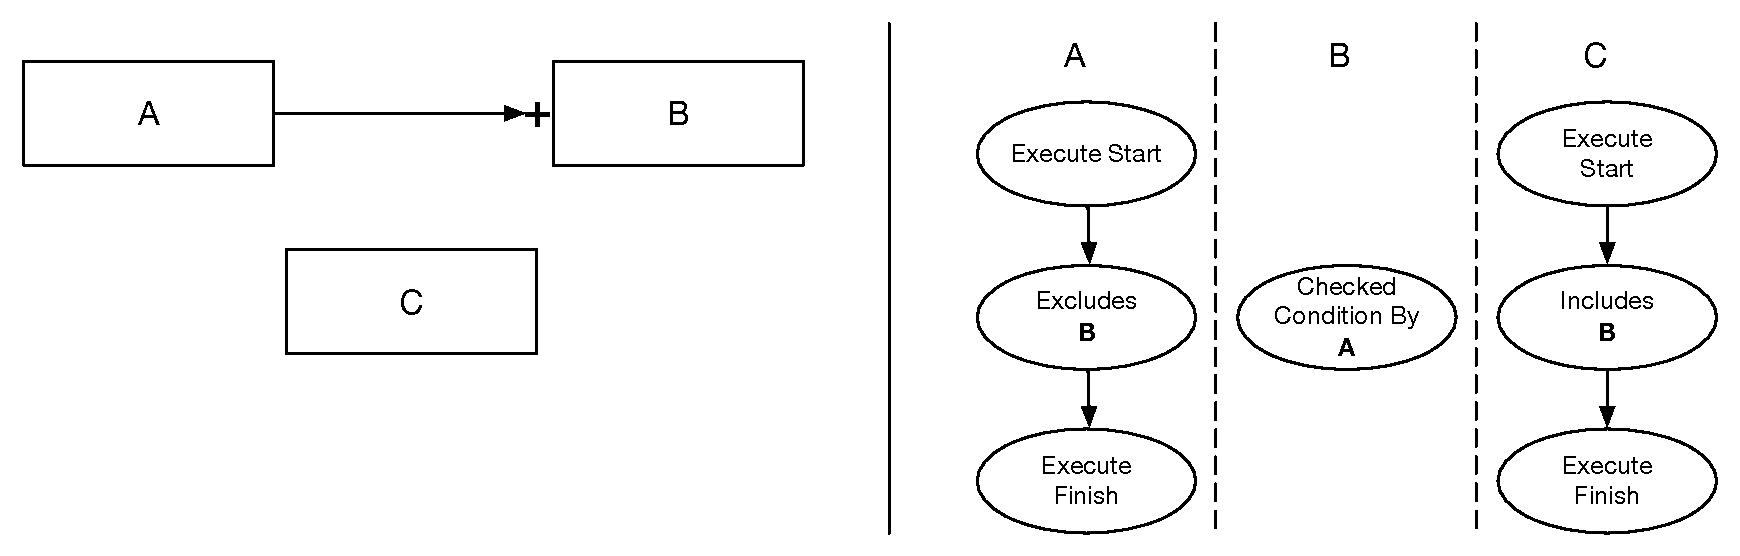
\includegraphics[width=\textwidth]{5validation/images/only-specified-relations.pdf}
		\caption{A DCR graph and three examples of local histories violating \autoref{rule:validrelations}.}
		\label{fig:validation:only-specified-relations}
	\end{figure}
	
	\noindent It can be validated that local histories adhere to \autoref{rule:validrelations} by examining every action, and for each outgoing and incoming action, the event, its counterpart, and action type must be present in the rules of the workflow.
	
	\begin{ruledef}
		\textbf{Only complete executions}: A given event, $E$, must have actions for each of its outgoing relations when executing. Each of the counterparts of these actions must have a corresponding action in their history after $E$ has executed. For any execution there must be exactly one action of type \textup{Execute start} happening before a single action of type \textup{Execute finish}.
		\label{rule:completeexecutions}
	\end{ruledef}

	\begin{figure}[H]
		\centering
		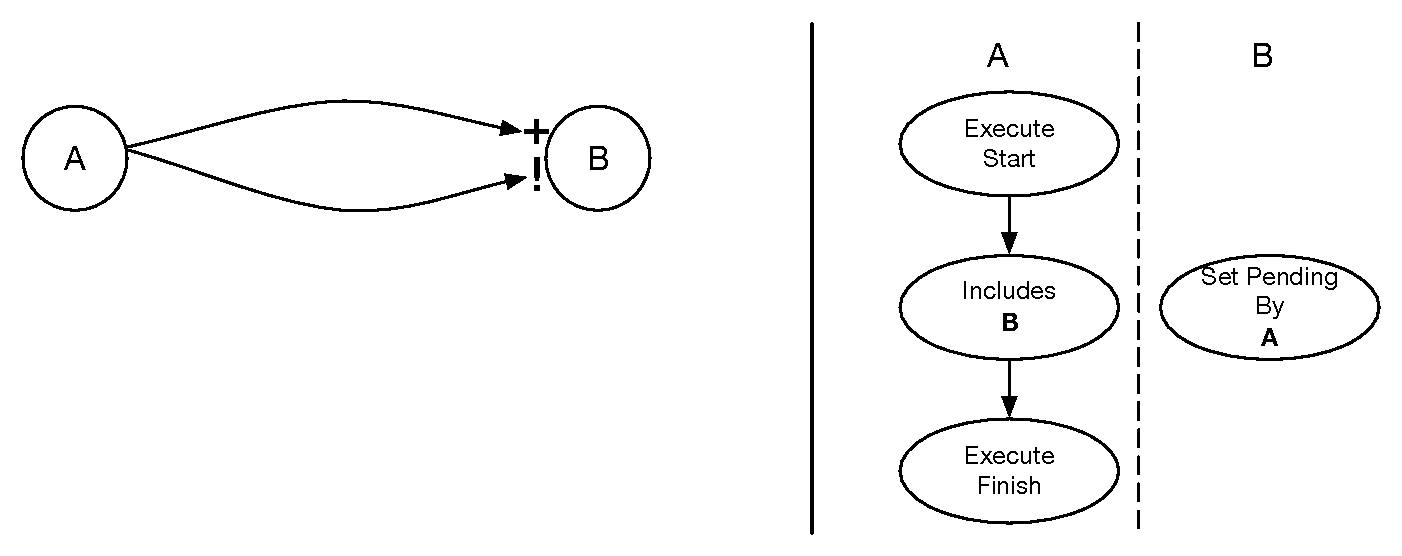
\includegraphics[width=\textwidth]{5validation/images/only-complete-executions.pdf}
		\caption{A DCR graph and two examples of local histories violating \autoref{rule:completeexecutions}.}
		\label{fig:validation:only-complete-executions}
	\end{figure}

	\noindent In \autoref{fig:validation:only-complete-executions} event $A$ does not contain an outgoing action of type \textit{Sets pending} and event $B$ does not contain an incoming action of type \textit{Included by}.

	\newpar In order to validate \autoref{rule:completeexecutions} for outgoing relations the following approach is taken: When an action of type \textit{Execute start} is encountered in the local history, a set of required actions for the execution is created from the rules of the workflow.
	
	For example, if event $A$ includes event $B$ and excludes itself, this set must contain an outgoing action corresponding to the inclusion of $B$, and two actions, one outgoing and one incoming, corresponding to the exclusion of event $A$ itself.
	
	Each consecutive action in the history, must be one of the actions in the set. The action is then removed from the set. When the set is empty, the next action in the history must have type \textit{Execute finish}.
	
	\newpar In order to validate \autoref{rule:completeexecutions} for incoming relations where the counterpart is not the event iself the following approach is taken: When an incoming action from an event $A$ is found, all actions corresponding to the remaining rules that specify that $A$ has a relation to the current event, is added. While the set is not empty, the consecutive actions in the history must exist in the set. An action is removed from the set when it is encountered.

	\begin{ruledef}
		\textbf{Executions only in Valid States}: The history of an event must only contain executions when the event is executable. This implies that the entirety of the history must match a run of the DCR graph it represents.
		\label{rule:executionvalidstate}
	\end{ruledef}
	
	\noindent Checking for this kind of inconsistency is nontrivial. A method of doing so is described in \autoref{sec:historyindcr:simulation}.
	
	\subsection{Serial Equivalence Rules}
	A given execution must comply to the rules of serial equivalence. That includes the following:
	
	\begin{ruledef}
		\textbf{Only non-disrupted executions}: A given event, $E$ must not contain ingoing relations or execute starts when already executing. Furthermore if an execution is started, it must also finish. The exception to the rule of ingoing relations is when an event has a relation to itself in which case that incoming action is allowed.
		\label{rule:non-disruptedexecutions}
	\end{ruledef}
	
	\noindent Figure \ref{fig:validation:only-non-disrupted-executions} shows an example where an execution of event $A$ is interrupted by an incoming action from another event.
	
	\begin{figure}[H]
		\centering
		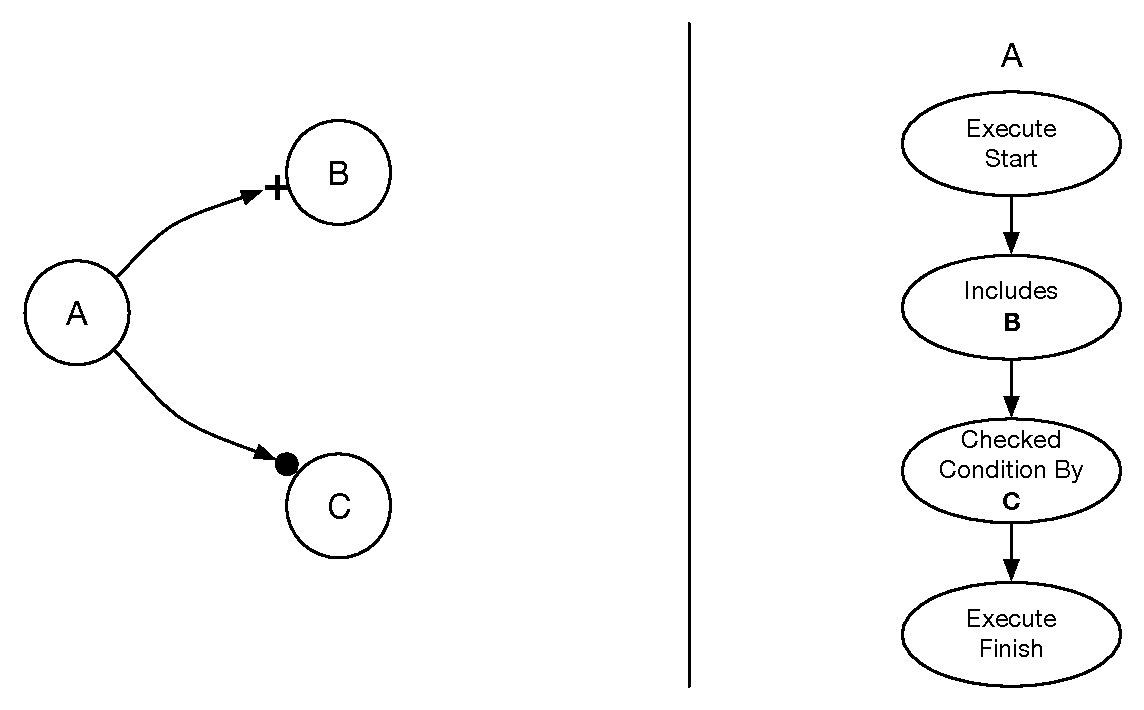
\includegraphics[width=.7\textwidth]{5validation/images/only-nondisrupted-executions.pdf}
		\caption{A DCR graph and an example of a history where \autoref{rule:non-disruptedexecutions} is violated}
		\label{fig:validation:only-non-disrupted-executions}
	\end{figure}
		
	\noindent The algorithm used to check \autoref{rule:completeexecutions} for outgoing relations is also used to check \autoref{rule:non-disruptedexecutions}.
	
	\begin{ruledef}
		\textbf{Wait for complete execution}: A given event, $A$ must be affected by all its ingoing relations from an event, $B$ when $B$ executes before anything else happens. The exception to the rule is when an event has a relation to itself in which case actions from the execution are allowed before the next incoming action happens. 
		\label{rule:wait-for-complete-execution}
	\end{ruledef}
	
	\noindent Figure \ref{fig:validation:wait-for-complete-execution} shows a situation where $B$ is included by $A$ but executes before the response relation from $A$ is present in the history.
	
	\begin{figure}[H]
		\centering
		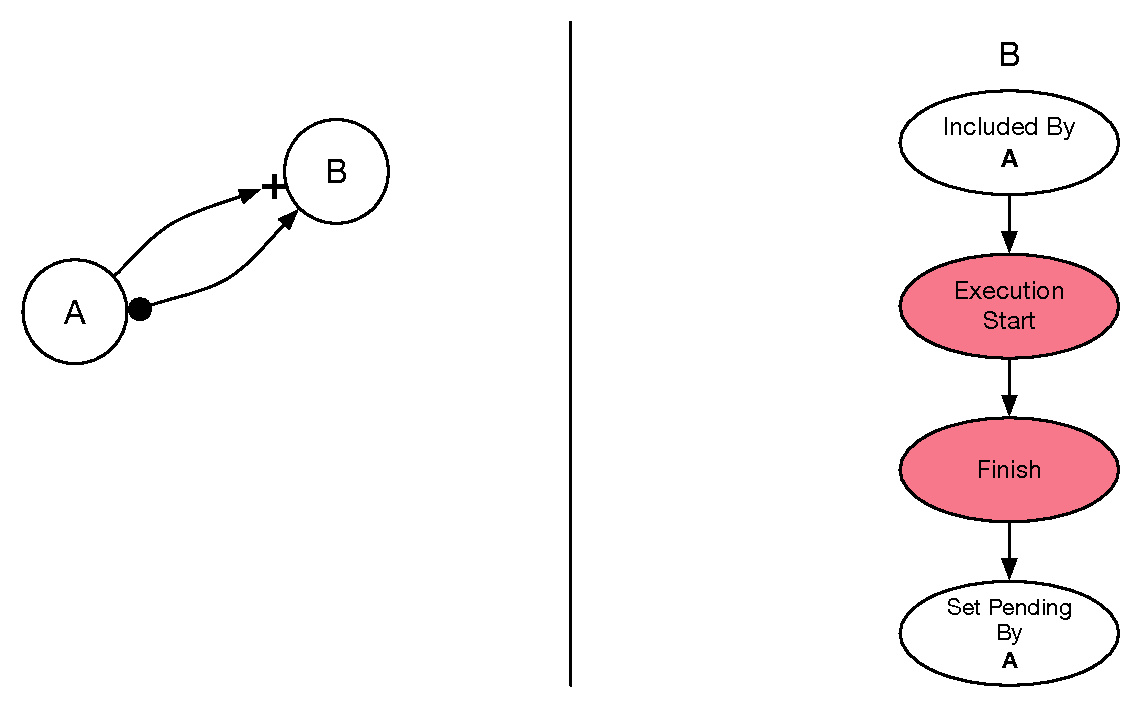
\includegraphics[width=.7\textwidth]{5validation/images/wait-for-complete-execution.pdf}
		\caption{A DCR graph and an example of a history where \autoref{rule:wait-for-complete-execution} is violated}
		\label{fig:validation:wait-for-complete-execution}
	\end{figure}
	
	\noindent The algorithm used to check \autoref{rule:completeexecutions} for incoming relations is also used to check \autoref{rule:non-disruptedexecutions}.
	
	\subsection{Lamport's Logical Clocks}
	A given history must conform to the rules of Lamport's logical clocks. That includes the following:
	
	\begin{ruledef}
		\textbf{Total Order of Timestamps}: Every action in the local history of an event must have a timestamp less than the timestamp of any action it happens before.
		\label{rule:total-order-timestamps}
	\end{ruledef}
	
	\noindent This kind of inconsistency can be checked by examining each action on a single event. If the timestamps are not increasing for each edge in the graph then the event must be cheating.
	
	\begin{ruledef}
		\textbf{Message Exchange Timestamp Order}: For every pair of actions that represent a message exchange, the timestamp of the outgoing action must be less than the timestamp of the incoming action.
		\label{rule:message-exchange-timestamp-order}
	\end{ruledef}
	
	\noindent A validation of this kind of inconsistency can be done on the history of each event. If the counterpart timestamps of the outgoing actions are not larger than the timestamps then the event is malicious. For incoming actions the counterpart timestamp must be less than the timestamp.
	
	\begin{ruledef}
		\textbf{Total Order of Counterpart Timestamps}: In the local history of an event, actions with the same counterpart ID must have a counterpart timestamp less than the counterpart timestamp of all other actions with the same counterpart ID that it happened before. The exception to the rule is when an event has a relation to itself in which case counterpart timestamp can be one lower.
		\label{rule:total-order-counterpart-timestamps}
	\end{ruledef}
	
	\noindent A validation of this kind of inconsistency can be done on each single event. Since each incoming and outgoing action must have a counterpart, it is possible to keep a mapping between counterparts and the last timestamp that counterpart had. Recall that the implementation requires that all correct processes only accept higher timestamps for a counterpart, than any timestamp seen from that counterpart before. \todo{Husk at skrive dette!} If a new timestamp for a counterpart is lower than the previous, then the event must be malicious.
	
	\newpar Because histories are represented as directed acyclic graphs, cycles must not exist. Rule \ref{rule:total-order-timestamps} and \ref{rule:message-exchange-timestamp-order} makes it possible to observe cycles and identify the local histories from where the cycles originate.
	
	Together, these rules make sure that no cycles can exist. If an action happens before another action with a lower timestamp, at least one of rules \ref{rule:total-order-timestamps} and \ref{rule:message-exchange-timestamp-order} have been violated. Examples of violations of rules \ref{rule:total-order-timestamps} and \ref{rule:message-exchange-timestamp-order} are shown in figures \ref{fig:validation:message-exchange-timestamp-order-cycle} and \ref{fig:validation:message-exchange-timestamp-order-cycle}.
	
    \begin{figure}[H]
		\centering
    	\begin{minipage}{.45\textwidth}
			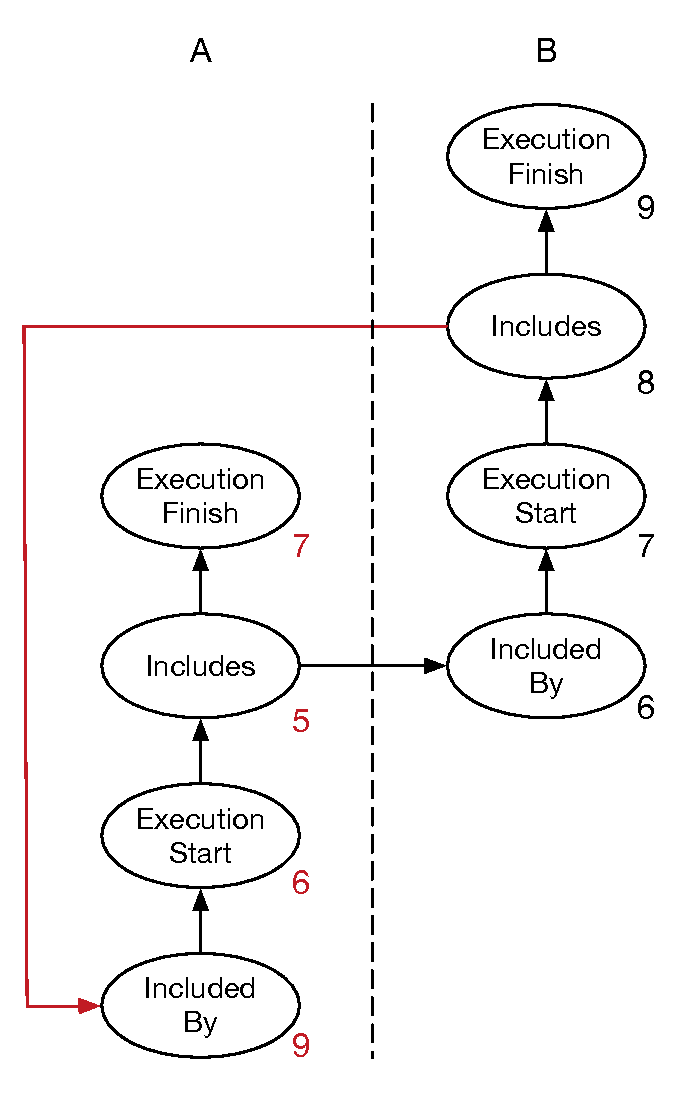
\includegraphics[width=.89\textwidth]{5validation/images/total-order-of-timestamps-cycle.pdf}
			\caption{An example of two histories forming a cycle by violation of \autoref{rule:total-order-timestamps}.}
			\label{fig:validation:total-order-of-timestamps-cycle}
    	\end{minipage}
		\hfill
		\begin{minipage}{.45\textwidth}
	    	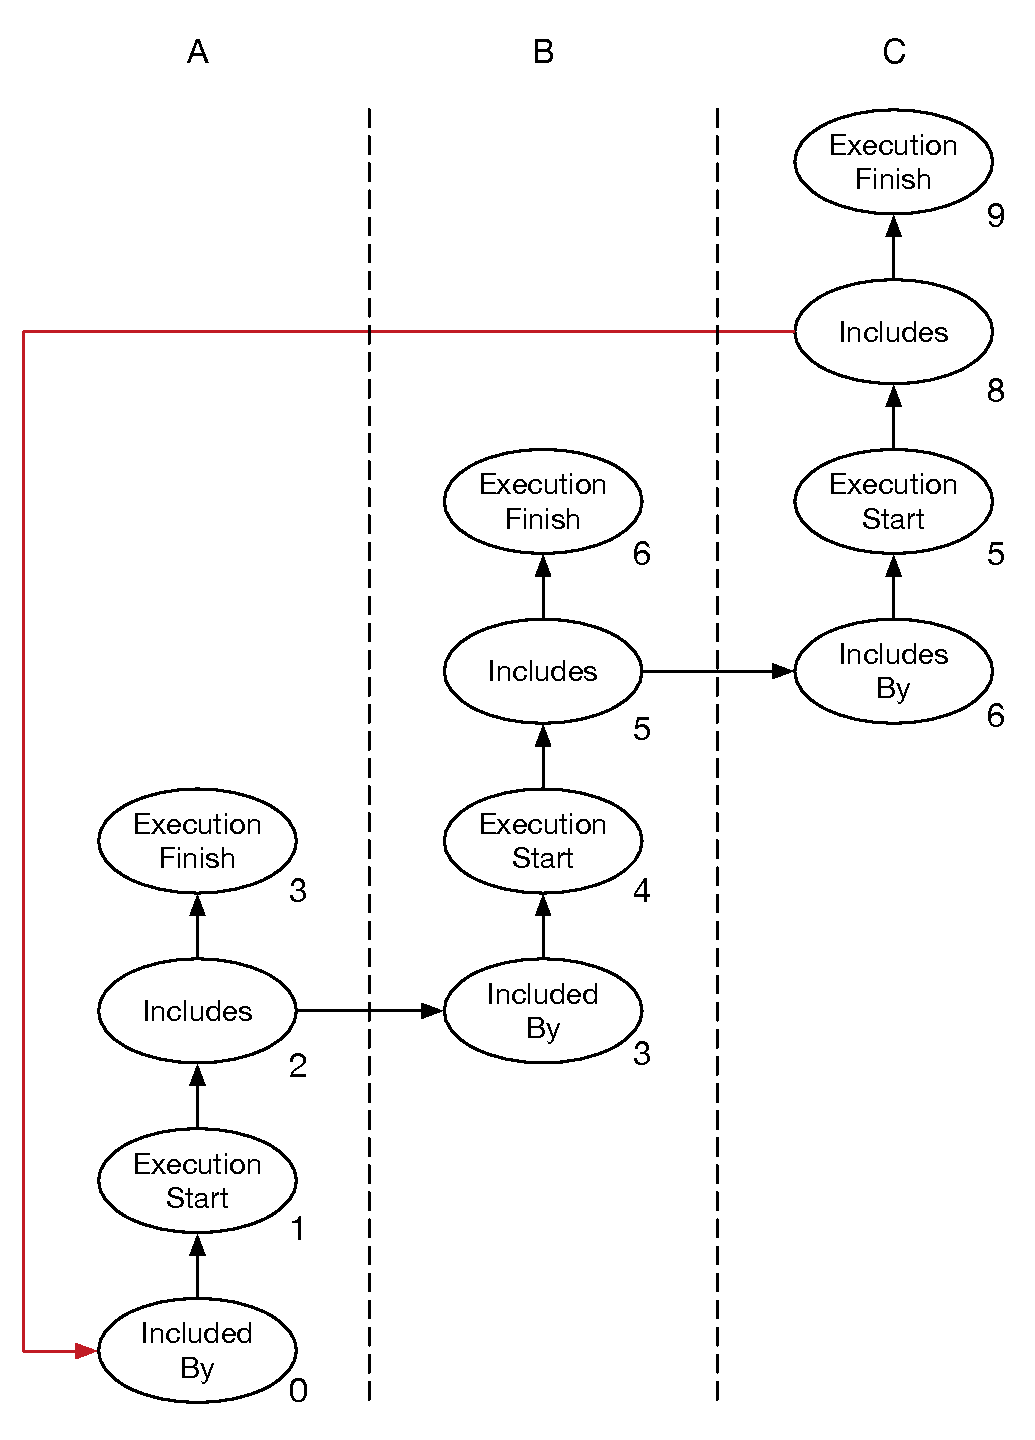
\includegraphics[width=\textwidth]{5validation/images/message-exchange-timestamp-order-cycle.pdf}
	    	\caption{An example of three histories forming a cycle by violation of \autoref{rule:message-exchange-timestamp-order}.}
	    	\label{fig:validation:message-exchange-timestamp-order-cycle}
		\end{minipage}
	\end{figure}
	
	\noindent On \autoref{fig:validation:total-order-of-timestamps-cycle} a cycle is created when event $A$ changes the order of its actions, violating \autoref{rule:total-order-timestamps} while still keeping the timestamps of message exchanges in an increasing order.
	
	\newpar On \autoref{fig:validation:message-exchange-timestamp-order-cycle} a cycle is created when timestamps of message exchanges are not kept in an increasing order, violating \autoref{rule:message-exchange-timestamp-order}. The timestamps of actions in the local histories are in increasing order which means that \autoref{rule:total-order-timestamps} is not violated.
	
	\section{Consistent Cheating}
	Until now we have examined inconsistent cheating, but malicious events are also able to cheat consistently:

	\newpar Consistent cheating can take a number of forms:

	\begin{ruledef}
		\textbf{Incorrect timestamps}: A malicious event manipulates the timestamps of the actions in the history, while still being in accordance to Lamport's logical clocks
	\end{ruledef}
	
	\figuretodo{to historikker der er ens bortset fra timestamps}
	The only actions which more that one event know of are the action which are part of a relation. The consequence of this is that it is only possible to check if events disagree on the timestamps of these actions and not the rest. To make this validation each ingoing action is matched with outgoing actions and if it is not possible to find a match, one of the events must be malicious. 
	
	\begin{ruledef}
		\textbf{Incorrect number of executions}: The history of a malicious event states that it has executed either fewer or more times than it has done.		
	\end{ruledef}

	\figuretodo{to historikker hvor antallet af executions ikke matcher}
	To check for this kind of cheating each pair of events that have relations are examined. If event A and event B is examined, then the amount of every outgoing action from A to B must match the amount of ingoing actions on B from A. If the amount does not match then one of the events must be malicious and vice versa.
	
	\begin{ruledef}
		\textbf{Incorrect number of incoming actions}: The history of a malicious event states that it has been affected either fewer or more times than what has happened.
	\end{ruledef}
	
	\figuretodo{to historikker hvor antallet af incoming groups ikke matcher }
	This type of cheating is already checked for by the method introduced in the previous paragraph.
	
	\newpar To argue that there are no other ways to consistently cheat it is necessary to examine what possible activities an event can take part of. 
	
	An event can execute or it can be affected by an execution. Not executing is just as valid as doing so (if the state of the workflow allows it). Furthermore, an action with a timestamp which is in accordance to Lamport's logical clocks can have another timestamp which is also in accordance. Therefore it is not possible to distinguish the correct timestamp from the incorrect. \todo[inline]{this paragraph has bullshit argumentation of the types being complete. plz help it}
	
	\subsection{Cases}
	Detecting and identifying consistently cheating events is difficult, because it is not possible to look at a single event's history and determine if it is valid or not. We will now examine how the structure of the DCR graph, and the connection between malicious events contribute to the ability to detect and identifying consistent cheating. The type of relation has no influence on the cases and relations are therefore visualised as a simple arrow from event to event.
	
	\newpar \textbf{Case 1 - Single Malicious Event}: In this case (see \ref{fig:consensus:single-malicious}), the event does not share relations with any other event, there is no one to disagree with any timestamps on actions and, in addition, completely oppose to the fact that an execution has happened or not. Therefore in workflows or subworkflows that include such events, it is not possible to identify or even observe if any kind of consistent cheating has happened.
	
	\begin{figure}[H]
		\centering
		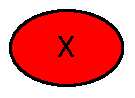
\includegraphics[]{5validation/images/1.pdf}
		\caption{}
		\label{fig:consensus:single-malicious}
	\end{figure}
	
	
	\newpar \textbf{Case 2 - Single Malicious Event With Relation to Self}: This case (see \ref{fig:consensus:single-malicious-with-relation}), just like case 1, in this case there are no one but the event itself to disrupt the cheating and therefore it is not possible to observe or identify consistent cheating.
	
	\begin{figure}[H]
		\centering
		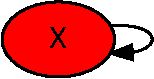
\includegraphics[]{5validation/images/5.pdf}
		\caption{}
		\label{fig:consensus:single-malicious-with-relation}
	\end{figure}
	
	\newpar \textbf{Case 3 - Single Malicious Event With Relation to Good Event}: In this case (see \ref{fig:consensus:single-malicious-with-good-relation}), the malicious event has a relation to a correctly working event. If the malicious event tries to cheat by changing the timestamps, it can do so in two ways. It can try to change the timestamps of the actions corresponding to the relation with the correctly working event, but in that case the two events will not agree on what happened and we are able to observe that one of them must cheat. Due to the fact that any of the two events could be malicious and change the timestamps it would not be possible to identify which of the two are evil.
	If the timestamp changes are on action which not related to the good event then it is not possible to observe nor identify. 
	\figuretodo{figur eksempler til tekst, der viser hvordan at to events kan være uenige}
	In the same way when looking at more or fewer executions, the relation action in the executions should have a counterpart but might not have. In the scenario where there are fewer executions the correctly working event will have actions with no counterpart and therefore it is only possible to observe and not identify this kind of cheating. 
	
	\begin{figure}[H]
		\centering
		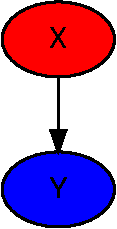
\includegraphics[]{5validation/images/3.pdf}
		\caption{}
		\label{fig:consensus:single-malicious-with-good-relation}
	\end{figure}
	
	\newpar \textbf{Case 4 - Single Good Event With Relation to Single Malicious Event}: In this case (see \ref{fig:consensus:single-good-with-malicious-relation}), a good event has a relation to a malicious event. Similarly to case 3 timestamp changes are observable due to the same factors, but instead of disagreeing on the outgoing relation in this case the malicious event will disagree on whether the good event executed or not. Due to the fact that when the malicious event executes the good event will not have any information about it, because it is not affected by that execution, the malicious event is able change the number of executions to its liking.
	\figuretodo{figur helt ens til den overfor men nu med den anden historik ond}
	 
	\begin{figure}[H]
		\centering
		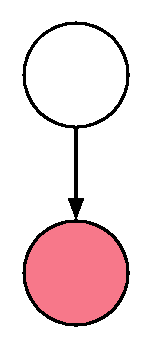
\includegraphics[]{5validation/images/2.pdf}
		\caption{}
		\label{fig:consensus:single-good-with-malicious-relation}
	\end{figure}
	
	\newpar \textbf{Case 5 - Single Good and Single Malicious Event with Relations to each other}: In this case (see \ref{fig:consensus:single-good-with-twoway-malicious-relation}), the situation is similar to that of case 3 and 4 in the sense that it provides the same ability to observe and the cheater.
	
	\begin{figure}[H]
		\centering
		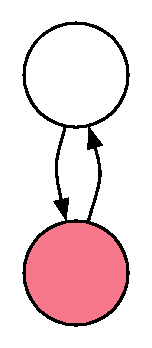
\includegraphics[]{5validation/images/6.pdf}
		\caption{}
		\label{fig:consensus:single-good-with-twoway-malicious-relation}
	\end{figure}
	
	\newpar \textbf{Case 6 - Single Malicious Event A with relation to Single Malicious Event B}: In this case (see \ref{fig:consensus:single-malicious-with-twoway-malicious-relation}), two malicious events work in collaboration to manipulate the data. Because a malicious event is also unpredictable, one of the events could function as a correctly functioning event and create the same depicting scenarios as in case 3 and 4, any absence of manipulation actually corresponds to the event functioning correctly.
	
	If it is assumed that both events work in collaboration to manipulate the history, it is both possible to change timestamps in such a way that it is not observable if they agree on the numbers, or observable if they disagree. Furthermore fewer or more executions is equally easily obscured if they agree on it.
	
	\figuretodo{figur: eksempel på hvordan de kan tilføje flere executions sammen}
	
	\begin{figure}[H]
		\centering
		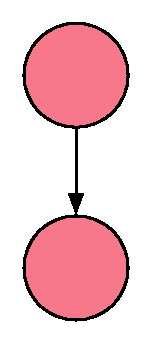
\includegraphics[]{5validation/images/4.pdf}
		\caption{}
		\label{fig:consensus:single-malicious-with-twoway-malicious-relation}
	\end{figure}
	
	\newpar \textbf{Case 7 - Two Malicious Events With Relations To Eachother}: In this case (see \ref{fig:consensus:two-malicious-with-twoway-malicious-relation}), two malicious events work in collaboration with to manipulate data with both their relations. This situation has the same properties as case 6.
	
	\begin{figure}[H]
		\centering
		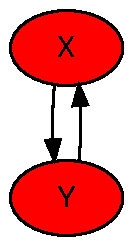
\includegraphics[]{5validation/images/7.pdf}
		\caption{}
		\label{fig:consensus:two-malicious-with-twoway-malicious-relation}
	\end{figure}
	
	\newpar In none of these cases it was possible to identify which of the events are malicious (in case 1 and 2 it is not possible to observe and therefore neither to identify). 
	
	This creates some interesting questions as to how one can try to identify which of the events are cheating. 
	One method could be to determine by counting how many of the neighbouring events disagree with you and if a majority disagrees the event will be marked as evil. Unfortunately that method has pitfalls since a good event with connection only to evil events could be marked as malicious. 
	
	If we require a new property of the DCR graph which states that in all neighbourhoods with $N$ events, a maximum of $N/2-1$ are malicious an election would not be able to falsely accuse a good event of being malicious. This property is commonly used for distributed systems which uses elections, but traditionally is only used to describe the amount of malicious nodes in the entire system. Therefore this property is more strict and perhaps more difficult to adhere to. 
	
	To worsen the situation substantially even if this property is adhered to, if an event is malicious does not mean that it is always malicious meaning it would be able to trick an election into not having a majority against it, so it is not possible to say that each event which disagrees with the values are malicious, which places us in the same situation to begin with, where we can only say one of two events must be malicious.
	
	\newpar It becomes apparent that the structure of the DCR graph has a great influence on whether it is possible to observe consistent cheating or not - especially in cases where a lot of malicious events are either interconnected or not connected to any other event at all it can be difficult to say anything about the state of the history. 
	
	One could argue what implications consistent cheating have on sub-graphs such as those of case 1 and 2, since their these events have little consequences on the rest of the workflow state. Therefore these events can only exist in two states (before and after they are executed) and therefore not being able to handle these kinds of situations is not that big a flaw. The major problems are apparent in situation 6 and 7 where, for example, a company can own a sub-part of the graph with many events working together to create a falsified image of what has actually happened. 
	
	\newpar Therefore a highly interconnected DCR graph is preferred if the users want to have a high probability of observing \todo{Fisk: Observing what?} 

    \section{Simulation}\label{sec:historyindcr:simulation}
    One of the more difficult validity properties to check is whether events have executed only when the state of the workflow allowed it. To do so, a lot of challenges must be addressed, it is not enough to check if the initial state of the event is executable, its conditions also need to be taken into perspective, furthermore the state of the workflow most likely changes over time with each execution. In addition since the history is a strictly partially ordered set, some executions happen concurrently which does not match physical time in which the events have executed.\todo[inline]{Jeg har lidt svært ved at indlede dette afsnit, men jeg synes ikke det skal starte med at det her er sværere end de andre validations.}
    
    \newpar One approach to this problem is to simulate the executions of the workflow. To do so, it is required that the rules of the workflow and the initial state of every event in the workflow is known. Furthermore it is required that an order of execution has been found, this is examined in the next chapter but we assume it is available. 
    
    Given the order of execution each execution has either zero or more ingoing edges. Each ingoing edge states which executions must have happened before, therefore an execution can first happen when all of its ingoing edges have executed. Therefore each execution have a counter based on the amount of ingoing edges which can be decreased each time one of the ingoing edges executes. An order of execution based on a valid history will always have some executions which have no ingoing edges since no cycles appear and some events \todo{executions? eller?}must happen before all their relations.
    
    \newpar To check if the execution of an event is possible, it is checked if the event is included and that the state of every condition of the event is either excluded or executed.\todo[inline]{Behøver vi skrive hvad det vil sige at være executable?} If the event was executable, the state of the workflow is changed according to the rules of the workflow.\todo[inline]{Vi opdaterer også state selvom den ikke er executable}
    
    \newpar To simulate the entire order of execution, the executions are checked for their ability to execute in a topological order. One way to create a topological order from an order of execution is to map each of the executions to the amount of executions that happens directly before an execution itself. An execution can be chosen as the next if and only if its counter reaches 0. When an execution is chosen, all of the executions it happens before has their counter decremented by 1. The order of which executions have happened are adhered to, but concurrent executions happen in a random order.\todo[inline]{Mikael: Jeg har omskrevet det her lidt, men ladet nogle sætninger være. Check gerne at det giver mening}
    
    Executions can only be concurrent if the events they belong to do not share outgoing relations. If two events share outgoing relations, one of them must affect the shared event before the other and an order would be able to be created. Therefore in an order of execution only one of the ingoing edges can be of an ingoing relation, the rest must be based on outgoing relations which can determine that the execution happens after some other execution. The order of which concurrent executions are simulated therefore does not matter since they order of which they execute can only result in one state change which affects common outgoing edges.\todo[inline]{hvad siger vi her?}
    
    \newpar If an execution was not executable, it is possible to identify if it is the event itself which is malicious or if it is one or more of the condition events. If the state of the event was not executable then the event must be malicious, note that the conditions in this case also could be malicious. If the state is executable and the conditions are included and not executed, another situation arises. The conditions could have returned false information to the executing event, or the executing event could have executed regardless of the values returned. Therefore in this case only a set of possible malicious events can be determined.\todo[inline]{Mikael: Jeg har svært ved at forstå hvad vi vil med denne paragraf. Måske en figur kan hjælpe?}
    \todo[inline]{Fisk: Jeg har generelt at forstå det her afsnit. Det skal vi nok lige gå igennem igen.}

	\newpar In \autoref{alg:simulation} the simulation algorithm can be seen. It runs in time linear to the amount of executions.
	
	\figuretodo{figur over en order of executions med counters på hver executions - eventuelt en ekstra med hvordan det ser ud efter at x events har executed. Mikael: For mig er det ikke det essentielle ved algoritmen "Simulation".}
	
	\begin{algorithm}[H]
		\begin{algorithmic}
			\Function{Simulation}{orderOfExecution, DCRRules, state}
			\State orderedExecutions $\leftarrow$ \Call{TopilogicalSort}{orderOfExecution} \Comment Returns a queue
			\State failures $\leftarrow$ List.Empty
			\While{not orderedExecutions.isEmpty}
				\State execution $\leftarrow$ \Call{Queue.Pop}{orderedExecutions}
					\If{not \Call{IsExecutable}{execution.Event, state}}
					\State failures $\leftarrow$ \Call{List.Add}{execution, failures}
				\EndIf
				\State state $\leftarrow$ \Call{ApplyExecution}{execution.Event, DCRRules, state}
			\EndWhile
			\State\Return failures
			\EndFunction
		\end{algorithmic}
		\caption{The \textbf{Simulation} algorithm}
		\label{alg:simulation}
	\end{algorithm}
	\todo[inline]{Check lige op på algoritmen generelt}
	
	\newpar This algorithm is based on the forward chaining algorithm of entailment in propositional theorem proving\todo{ref section 7.5 in SISP bog. Mikael: Jeg synes det er fedt at vi har anvendt viden fra det fag, men synes at det stikker lidt uden for de ting vi har sagt er nødvendigt for at forstå denne opgave. Jeg har også forsøgt at formulere i teksten ovenfor hvordan man kan anvende algoritmen til at finde denne order, men uden at gå alt for teknisk til værks.}, which also runs in linear time and is used to see if a knowledge base can entail a proposition.
	
    \newpar There is a couple of challenges and approaches to how it is handled both if cheating has been observed before the simulation or cheating is observed during the simulation. We have chosen the approach to mark if an execution was inconsistent, but allow it to "execute" and then change the state to see if the rest of the order of execution was consistent. One could easily check the rest of the order of execution without the state change of the inconsistent execution to see what implications that cheating could have had.
    
    \todo[inline]{Flyttet fra Background herfra...}
    The reason why typical Byzantine general problem algorithms cannot be used in this project is that the commander needs to use information from the potentially malicious processes to decide on a correct value to propose. Again since at most two events share the information the requirement that maximum $f=N/3$ malicious is not kept in regards to information gathering and it is therefore impossible to get ensure correct information from each event.\todo{måske er der noget af det her der skal rykkes ned i validation og election så vi faktisk bare beskriver hvad det er.}
    Furthermore, most consensus algorithms require all processes of the election to be able to propose a value which should be agreed upon, but since each DCR event does not know nor is able to produce the entire history of the workflow, and therefore cannot propose a value which other events would be able to agree on, such algorithms cannot be used.\todo[inline]{... Flyttet fra Background hertil}
    
    \section{Observability and identifiability}
    
    \section{Correctness}
    Note that property 1 must be violated in order to violate either property 2, 3, or 4. 
    
    If it is possible to detect both consistent and inconsistent cheating, then it is possible to decide if a history is valid or invalid.